\documentclass[12pt, a4paper]{article}

\usepackage{ctex}[ubuntu]
\usepackage{amsmath}
\usepackage{graphicx}

\newcommand\tab[1][1cm]{\hspace*{#1}}

\title{ItemCF推荐系统的MapReduce实现}

\author{劳马东  16337113\\计算机科学与技术(超算方向)}
\date{\today}

\begin{document}
\maketitle
\rmfamily

\section{ItemCF的基本思想}
\begin{enumerate}
  \item 计算物与物之前的相似度
  \item 根据用户的行为历史,给出和历史列表中的物品相似度最高的推荐
\end{enumerate}
\par 通俗的来讲就是:
\ttfamily
\par 对于物品A,根据所有用户的历史偏好,喜欢物品 A 的用户都喜欢物品 C,得出物品 A 和物品 C 比
较相似,而用户 C 喜欢物品 A,那么可以推断出用户 C 可能也喜欢物品 C。
\rmfamily
\section{算法实现步骤}
\subsection{数据集}
数据格式:$User\_id,Item\_id,preference$
数据集字段:
\begin{itemize}
  \item $User\_id$: 用户ID
  \item $Item\_id$: 物品ID
  \item $preference$: 用户对该物品的评分
\end{itemize}
\begin{figure}[ht]
\centering
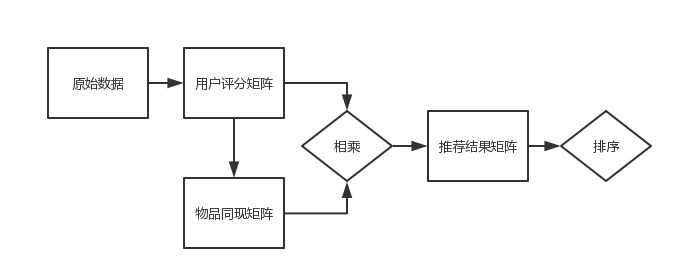
\includegraphics[scale=0.5]{steps.jpg}
\caption{ItemCF实现步骤}
\label{fig:label}
\end{figure}
\subsection{计算用户评分矩阵$P$}
假设有n个用户和m个物品,则
\begin{equation}       %开始数学环境
P =
\left(
  \begin{array}{ccccc}
    p_{11}  & p_{12}  & p_{13}  & ... & p_{1m}\\
    p_{21}  & p_{22}  & p_{23}  & ... & p_{2m}\\
    p_{31}  & p_{32}  & p_{33}  & ... & p_{3m}\\
    ...     & ...     & ...     & ... & ...\\
    p_{n1}  & p_{n2}  & p_{n3}  & ... & p_{nm}
  \end{array}
\right)
\end{equation}
\par 其中$p_{ij}$($i \in [1,n], j \in [1,m]$)代表用户i对物品j的评分。
\par 从行的方向看,S的每一个行在MapReduce程序中可以用一行简单的字符串来表示:
\begin{equation}
  User\_id_i \tab Item\_id_1:p_{i1},Item\_id_2:p_{i2},...,Item\_id_j:p_{ij},...
\end{equation}
\par 因此,该步骤可以简单归纳如下, 代码如图2、3:
\begin{enumerate}
  \item 在map阶段,分割每行内容,输出的key为$User\_id_i$,value为$Item\_id_j:p_{ij}$
  \item 在reduce阶段,将User\_id相同的所有评分记录进行汇总,输出的key仍然为$User\_id_i$,
  value形如:$Item\_id_1:p_{i1},Item\_id_2:p_{i2},...,Item\_id_j:p_{ij},...$
\end{enumerate}
\begin{figure}[ht]
\centering
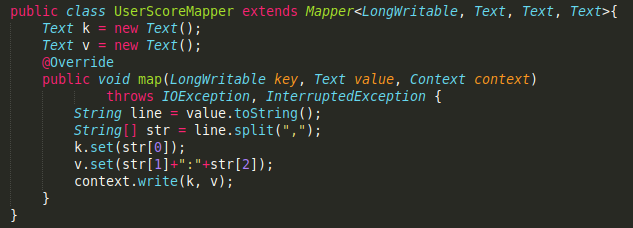
\includegraphics[scale=0.5]{m1.png}
\caption{用户评分矩阵-map}
\end{figure}

\begin{figure}[ht]
\centering
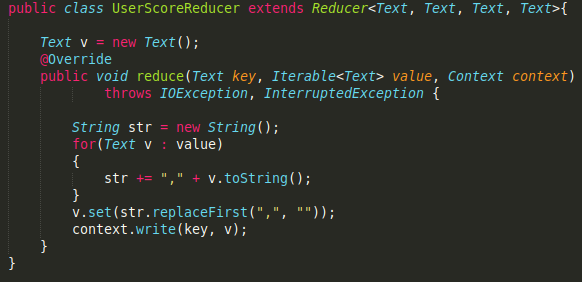
\includegraphics[scale=0.5]{r1.png}
\caption{用户评分矩阵-reduce}
\end{figure}

\subsection{计算物品同现矩阵$T$}
T是由上一步得到的结果计算而来的,具体而言就是将文件中格式为“$User\_id_i \tab Item\_id_1:p_{i1},
Item\_id_2:p_{i2},...,Item\_id_j:p_{ij},...$”的行转化成格式为“$Item\_id_k:Item\_id_l\tab$次数”
的行。
\begin{equation}       %开始数学环境
T =
\left(
  \begin{array}{ccccc}
    t_{11}  & t_{12}  & t_{13}  & ... & t_{1m}\\
    t_{21}  & t_{22}  & t_{23}  & ... & t_{2m}\\
    t_{31}  & t_{32}  & t_{33}  & ... & t_{3m}\\
    ...     & ...     & ...     & ... & ...\\
    t_{m1}  & t_{m2}  & t_{m3}  & ... & t_{mm}
  \end{array}
\right)
\end{equation}
\par $t_{ij}$($i \in [1,m], j \in [1,m]$)代表物品i和物品j同时被用户使用过的次数和,即:
\begin{equation}
  t_{ij} = \sum_{k=1}^n Item\_id_i \in a_k \land Item\_id_i \in a_k
\end{equation}
\par 其中$a_k$表示用户k使用过的物品的集合。这个矩阵的意义就是各个物品之间的相似度,为什么可以这么说?
如果两个物品经常同时被很多用户喜欢,那么可以说这两个物品是相似的,同时被越多的用户喜欢,
T中相应的值就越大,这两个物品的相似度就越高。
\par 因此,该步骤可以简单归纳如下:
\begin{enumerate}
  \item 在map阶段,枚举每行内容中的Item\_id,输出的key为$Item\_id_i:Item\_id_j$,value为1,
  代码如图4
  \item 在reduce阶段所做的就是根据key对value进行累加输出
\end{enumerate}
\par map阶段两两枚举某个用户使用过的物品,生成$(item_i, item_j, 1)$项。
\begin{figure}[ht]
\centering
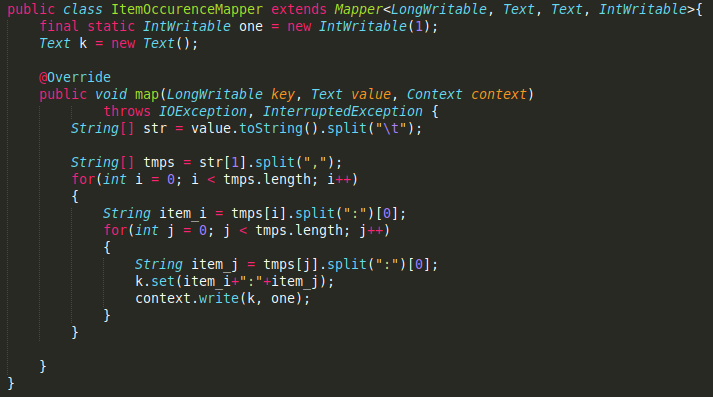
\includegraphics[scale=0.5]{m2.png}
\caption{物品同现矩阵-map}
\end{figure}

\newpage
\subsection{计算推荐结果矩阵$R$}
\begin{equation}
  R = P \times T
\end{equation}
\par $R_{ij}$表示用户i对物品j的喜好度(推荐结果)。为什么两个矩阵相乘可以得到推荐结果?
因为其他用户对物品1的评价*物品1与物品2的相似度,可以大致反映出用户对物品2的喜好度。
\par 该步骤可以简单归纳如下, 代码如图5、6:
\begin{enumerate}
  \item 在map阶段,输入的value为S中的一行,将其与T中的每一列相乘得到R中的一行,
  并筛选出未被其使用过的物品及对应的喜好度
  \item 在reduce阶段,输出map阶段筛选的结果,key为$User\_id_i$,value为$Item\_id_j:R_{ij}$
\end{enumerate}
\begin{figure}[ht]
\centering
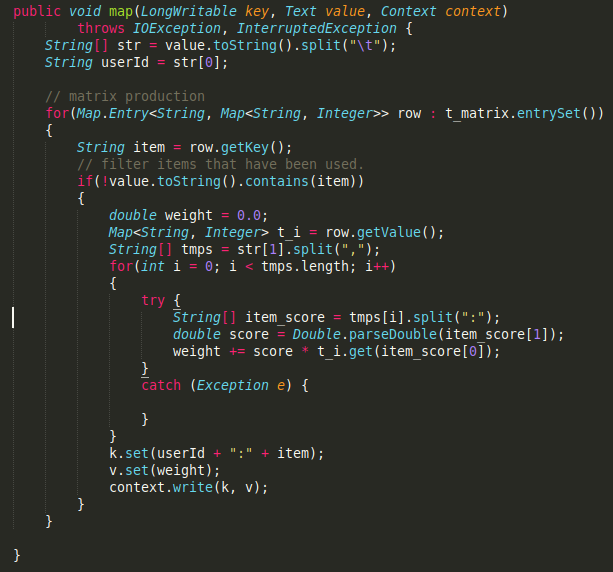
\includegraphics[scale=0.5]{m3.png}
\caption{推荐结果矩阵-map}
\end{figure}

\begin{figure}[ht]
\centering
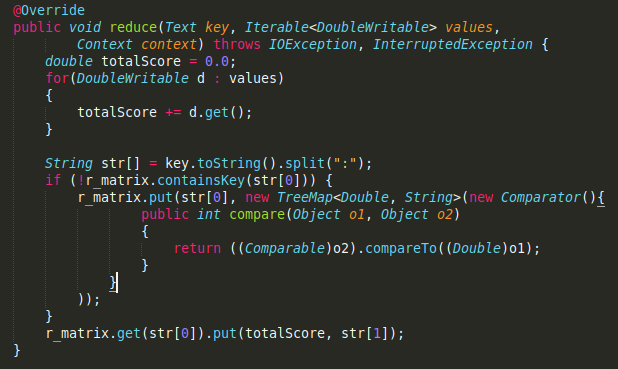
\includegraphics[scale=0.5]{r3.png}
\caption{reduce}
\end{figure}
\subsection{对推荐结果按推荐分值从高到低排序}
排序是为了方便挑选出用户最有可能喜欢的一些物品,因为物品的总数很多,不可能把所有物品都推荐
给用户。推荐物品个数可以是一个设定的值,由于上一步的map阶段已经筛选出了用户所有未使用过
的物品,可以考虑在reduce将结果存入一个从大到小排序的TreeMap中。代码如图6、7:
\begin{figure}[ht]
\centering
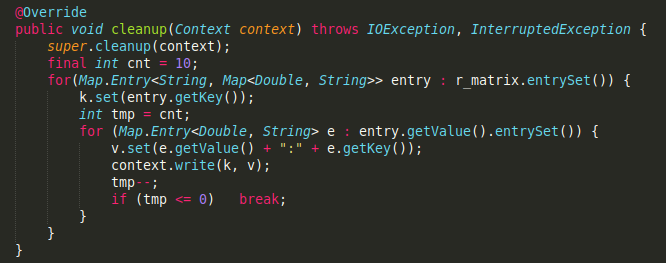
\includegraphics[scale=0.5]{recommend10.png}
\caption{选择top10推荐结果}
\end{figure}
\section{测试结果}
测试数据集:ratings.csv(下载自https://grouplens.org/datasets/movielens/)
\par 测试环境:Ubuntu18.04 64位 hadoop 2.9.1
\par 结果:output文件夹中, user-score-matrix.txt为用户评分矩阵P, item-occurrence-matrix.txt
为物品共现矩阵T, result.txt为推荐结果。

\begin{thebibliography}{9}
\bibitem{Hadoop}
  87hbteo,
  \emph{Ubuntu16.04下hadoop的安装与配置(伪分布式环境)}.
  https://www.cnblogs.com/87hbteo/p/7606012.html

\bibitem{ItemCF1}
  liushahe2012,
  \emph{Hadoop案例之基于物品的协同过滤算法ItemCF}.
  https://blog.csdn.net/liushahe2012/article/details/54122080
\bibitem{ItemCF2}
  FreeBird,
  \emph{基于物品的协同过滤ItemCF的mapreduce实现 }.
  https://www.cnblogs.com/anny-1980/articles/3519555.html
\end{thebibliography}
\end{document}
